\documentclass{beamer}
\usepackage[spanish]{babel}
\usepackage[utf8]{inputenc}

%justificado
\usepackage{ragged2e}
\justifying

%tema
\usetheme{Warsaw}
\usecolortheme{default}
\setbeamercovered{transparent}

\title [Ingeniería en Software]{Personal Software Process - ISO/IEC 12207}
\author[Grupo 1]{Oscar León Trureo\\Sebastián Menéndez Sáez\\Claudio Piña Novoa}
\date{\today}
\institute[]{Universidad Tecnol\'ogica Metropolitana}
%\logo{}


%empieza el Documento
\begin{document}


\begin{frame}
	\maketitle
\end{frame}

\begin{frame}
	\frametitle{Índice}
	\tableofcontents[]
\end{frame}

\section{Personal Software Process}
		\subsection{Introducci\'on}
		
			\begin{frame}
				\begin{center}
					\begin{block}{}
						\begin{center}
							{\huge Personal Software Process}
						\end{center}
					\end{block}
				\end{center}
			\end{frame}			
		
			\begin{frame}{Introducci\'on}
				Dentro del mundo del desarrollo en Software, podemos encontrar las metodolog\'ias, las cuales son un conjunto de buenas pr\'acticas, las cuales nos permiten:\\ \pause
				\begin{itemize}
					\item Crear mejores aplicaciones.\pause
					\item Llevar un mejor proceso de desarrollo.\pause
					\item Agilizar el desarrollo en sí.\pause
					\item etc \ldots
				\end{itemize}				
			\end{frame}
			
			\begin{frame}{Introducci\'on}
				Existen una gran cantidad de metodologías, las cuales pueden estar enfocadas al desarrollo en sí, a la gestión, a la calidad, al desarrollador, como también puede ser una mezcla.\\
				\smallskip
				Personal Software Process, es una metodolog\'ia enfocada a la calidad del desarrollo del software a nivel personal, la cual se basa en factores que veremos más adelante.
			\end{frame}		
			
		\subsection{Historia}
			\begin{frame}{Historia}
				\pause
				\begin{itemize}
					\item Creado en el año 1995 por Watt's S. Humphrey en la Universidad de Carnegie Mellon, en Pittsburgh, Pennsylvania.\\ \pause
					\item El primer curso fue imparti\'o en la Universidad de Carnegie Mellon.\\ \pause
					\item fue plasmado en el libro ``A Discipline for SW Engineering'' de Humphrey.\\
				\end{itemize}
			\end{frame}
		
				\begin{frame}
					\begin{quotation}``La calidad del software está dada por la cantidad de procesos usados para desarrollarlo y mantenerlo''.\end{quotation}
			
				\hfill -- \parbox[t]{.9\textwidth}{Watts S. Humphrey,
				\textit{Creador de Personal Software Process}}

				\end{frame}
		
		\subsection{PSP}
			\begin{frame}{PSP}
				\textbf{Personal Software Process}, que en español significa \textbf{Proceso Personal de Software} (PSP), es un conjunto de buenas pr\'acticas las cuales se enfocan al control del tiempo y en la productividad de los Ingenieros en Software, ya sea en la mantencion de sistemas o en tareas de desarrollo.
				\\ \smallskip
				PSP fue diseñado para ayudar a los profesionales del software para que utilicen constantemente prácticas sanas de ingeniería del software, enseñándoles a planificar y dar seguimiento a un trabajo, utilizar un proceso bien definido y medido, a establecer metas mesurables y finalmente a rastrear constantemente para obtener las metas definidas.
			\end{frame}
			
			\begin{frame}{Principios de PSP}
				Personal Software Process, se caracteriza porque es de uso personal, es por esto que se definen principios enfocados a la individualidad:				
				\begin{itemize}
					\smallskip
					\item Cada ingeniero es diferente, para ser más eficiente, debe planificar su trabajo basándose en su experiencia personal.\\ \pause
					\item Cada ingeniero debe utilizar procesos bien definidos y mesurables.\\ \pause
					\item Los ingenieros deben asumir la responsabilidad personal de la calidad de sus productos.\\ \pause
					\item Cuanto antes se detecten y corrijan los errores, menor será el esfuerzo necesario para cumplir la meta.\\ \pause
					\item Es más efectivo prevenir los defectos, que detectarlos y corregirlos.\\
				\end{itemize}
			\end{frame}						
			
			\begin{frame}{PSP}
				\textbf{PSP} no es un est\'andar, es m\'as bien un alternativa que permite mejorar la forma en la que se construye el software, pero con un enfoque ``individual'', por lo que es muy recomendada para los desarrolladores que estén interesados en mejorar en lo que llamamos ``desarrollo individual''.
				\begin{figure}
    				\scalebox{0.2}{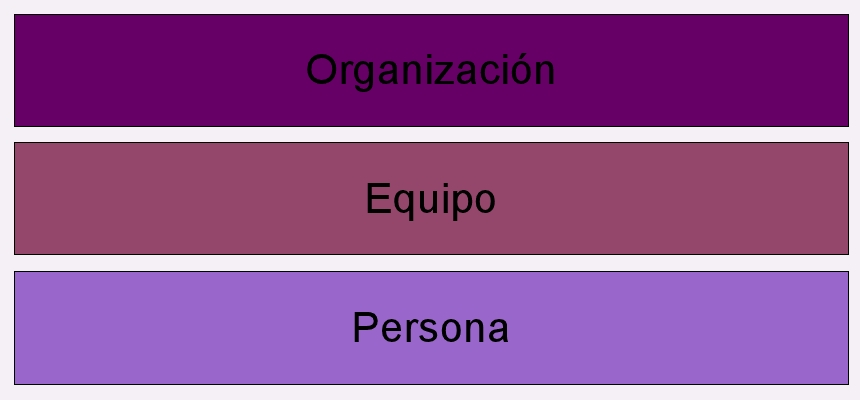
\includegraphics{Imagenes/Orga.jpg}} \caption{Niveles de la Organización}
				\end{figure}
			\end{frame}
				
			\begin{frame}{Pasos para la implementación de PSP}
				\begin{enumerate}
					\item Los ingenieros deben ser entrenados por un instructor calificado de PSP. \\ \smallskip \pause
					\item La Capacitacion es sobre grupos o equipos, y seran grupos que asi lo han sido y seguiran siendo. \\ \smallskip \pause
					\item Requiere un fuerte soporte de administración, en este sentido es necesario que los administradores entiendan PSP, saber como apoyarlos y como monitorear sus avances, sin un adecuado monitoreo los ingenieros caerán otra vez en los malos hábitos. \\ \smallskip \pause
					\item Después de ser bien entrenados y bien administrados lo que sigue es optimizar la interacción entre equipos y aquí entraría Team Software Process, el TSP extiende y refina los metodos de CMM y PSP sobre desarrollo y mantenimiento de equipos, y llegar a lo que se le llama un equipo autodirigido. \\ \smallskip
				\end{enumerate}
			\end{frame}
			
			\begin{frame}{Ciclo de Vida de PSP}
				Personal Software Process, tiene un ciclo de vida el cual consta de 5 fases principales, las cuales son fundamentales para el desarrollo de esta metodología: \\ \pause
				\begin{enumerate}		
					\item Planeación \pause
					\item Diseño de Alto Nivel \pause
					\item Revisión de Alto Nivel \pause
					\item Desarrollo Ciclico \pause
					\item Post Mortem
				\end{enumerate}
			\end{frame}											
				
			\begin{frame}{Fase de Planeación}
				\begin{block}{Entrada}
					Descripción del problema, resumen del proyecto, resumen cíclico, tamaño estimado, tiempo estimado, formas de planeación.
				\end{block}
				\begin{block}{Actividad}
					Requerimientos, tamaño estimado, desarrollo estrategia, estimados de recursos, planificación y programas de tareas, estimación de defectos.
				\end{block}
				\begin{block}{Salida}
					Diseño conceptual, resumen plan, resumen del ciclo, patrones de estimados de tamaño y planeación de tareas, programas de patrones de planeación, registro de tiempos.
				\end{block}
			\end{frame}
			
			\begin{frame}{Fase de Diseño de Producto}
				\begin{block}{Entrada}
					Tipificación requerimientos, diseño conceptual, patrones de estimaciones de tamaño, resumen parte ciclico, seguimiento.
				\end{block}
				\begin{block}{Actividad}
					Especificaciones externas, diseño modular, prototipos, estrategia de desarrollo y documentación, seguimiento.
				\end{block}
				\begin{block}{Salida}
					Diseño de programa, escenarios operacionales, especificación de funciones y lógica, resumen cíclico, seguimiento y estrategias de pruebas.
				\end{block}
			\end{frame}

			\begin{frame}{Fase Revisión o Validación del Diseño}
				\begin{block}{Entrada}
					Programa de diseño, escenarios operacionales, especificación de funciones y lógica, resumen ciclico, seguimiento y estrategia de pruebas y ciclo.
				\end{block}
				\begin{block}{Actividad}
					Diseño de apariencia, verificación de máquinas y lógica, consistencia del diseño, reuso, estrategia de verificación, detectar errores.
				\end{block}
				\begin{block}{Salida}
					Diseño de alto nivel, registro de seguimiento, tiempos y defectos.
				\end{block}
			\end{frame}
			
			\begin{frame}{Fase de Desarrollo o Implementación}
				\begin{block}{Entrada}
					Diseño de alto nivel, registro de seguimiento, tiempos y defectos, ciclo de desarrollo, estrategia de pruebas, patrones de operación y función.
				\end{block}
				\begin{block}{Actividad}
					Diseño de módulos, revisión de diseño, código, revisión de código, compilación, pruebas, aseguramiento de calidad y del ciclo.
				\end{block}
				\begin{block}{Salida}
					Modulos de sw, patrón de diseño, lista de verificación de código y diseño, resumen del ciclo, patrón de reporte de pruebas, registro de tiempo, defectos y seguimiento.
				\end{block}
			\end{frame}			
			
			\begin{frame}{Fase PostMortem, Evaluación Ciclo}
				\begin{block}{Entrada}
					Definición de problema y requerimientos, plan de proyecto y de ciclo, producto de software, patrón de diseño, lista de verificación de código y diseño, resumen del ciclo, patrón de reporte de pruebas, registro de tiempo, defectos y seguimiento.
				\end{block}
				\begin{block}{Actividad}
					Defectos previstos, removidos, tamaño, tiempo del producto.
				\end{block}
				\begin{block}{Salida}
					Producto, listas de verificación, plan de proyecto y ciclo, patrón de reporte de pruebas y diseño, forma con propuesta de mejora, registro seguimiento pruebas y tiempo.
				\end{block}
			\end{frame}				
					
			\begin{frame}{Ciclo de Vida}
				\begin{figure}								
					\scalebox{0.5}{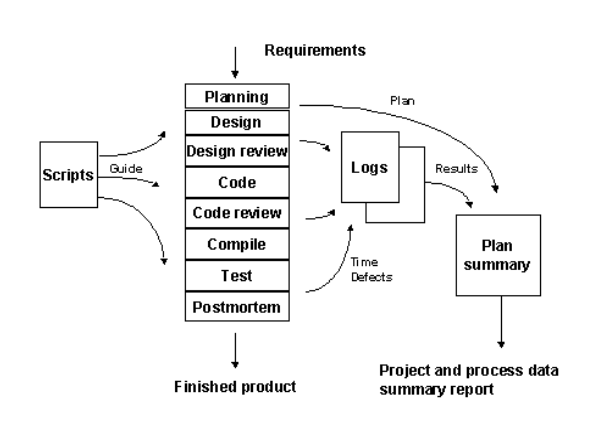
\includegraphics{Imagenes/Ciclo.png}} \caption{Ciclo de Vida PSP}
				\end{figure}			
			\end{frame}
			
			\begin{frame}{Requisitos}
				En está fase se definen los requisitos los cuales son definidos claramente en psp como:
					\begin{itemize}
						\item Descripción del problema.
						\item Especificación de componentes.
						\item Formas de procesos.
						\item Estimadores del tamaño del producto y tiempos en base a historicos.
					\end{itemize}
			\end{frame}					
			
			\begin{frame}{Ciclo de Vida}
				\begin{figure}								
					\scalebox{0.5}{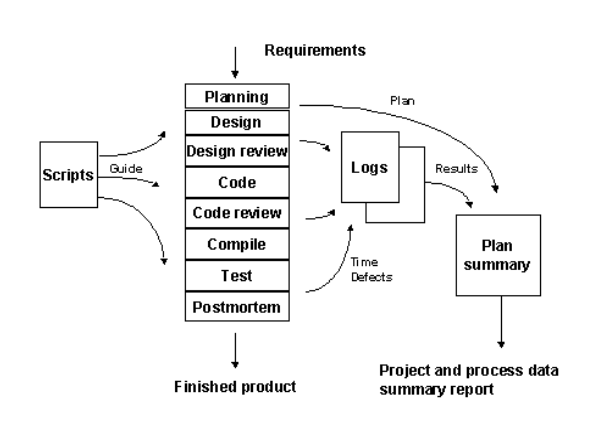
\includegraphics{Imagenes/Ciclo.png}} \caption{Ciclo de Vida PSP}
				\end{figure}			
			\end{frame}
			
			%%%%PSP%%%%			
			
			
			%%%%%ISO/IEC 12207%%%				
			
\section{ISO/IEC 12207}
		\subsection{Introducci\'on}
		
			\begin{frame}
				\begin{center}
					\begin{block}{}
						\begin{center}
							{\huge ISO/IEC 12207}
						\end{center}
					\end{block}
				\end{center}
			\end{frame}					
		
			\begin{frame}{Introducci\'on ISO}
				La ISO (Organización Internacional de Normalización), es el \textbf{organismo} encargado de promover el desarrollo de normas internacionales de fabricación (tanto de productos como de servicios), comercio y comunicación para todas las ramas industriales a excepción de la eléctrica y la electrónica. Su función principal es la de \textbf{buscar la estandarización de normas} de productos y seguridad para las empresas u organizaciones (públicas o privadas) a nivel internacional.\\ \smallskip
			\end{frame}
		
			\begin{frame}{Introducción IEC}
				La IEC (Comisión Electrotécnica Internacional), es una \textbf{organización} de normalización en los campos eléctricos, eléctronicos, y tecnologías relacionadas.\\ \smallskip
				A la IEC se le debe el desarrollo y difusión de los estandares para algunas unidades de medida tales como Gauss, Hercio, Weber; Así como la propuesta de una sistema de unidades estándar. Numerosas Normas se desarrollan en conjunto con la ISO (normas ISO/IEC).
			\end{frame}
			
			\subsection{Historia}
				\begin{frame}{Un poco de Historia}
					\begin{itemize}
						\item La norma surge a principios de la década de los noventa, como un estándar internacional.\pause
						\item Es una norma conjunta entre ISO e IEC.\pause
						\item Fue el Comité JTC1 quien construye la norma\pause
						\item Su principal motivación fue establecer un marco de trabajo común a la ingeniería del software. Aplicable a la Ingeniería y a la gestión.
					\end{itemize}
				\end{frame}
				\subsection{ISO/IEC12207}
				\begin{frame}{ISO/IEC 12207}
					\begin{definition}
						Es el estándar para los procesos de ciclo de vida del software de la organización ISO
					\end{definition}
				\end{frame}
				
				\begin{frame}{Ciclo de Vida del Software}
				\begin{center}
					\begin{center}
						{\huge Cu\'al es el Ciclo de Vida del Software?}
					\end{center}
					
					\begin{itemize}
					\pause
						\item Por concenso se toma en cuenta que el ciclo de vida de un software comienza en el momento que se concibe su idea o necesidad.\pause
						\item Luego es necesario comenzar a actuar de manera ortodoxa para describir el ámbito del problema y las soluciones posibles.\pause
						\item Para terminar, el ciclo comprende al desarrollo, mantenimiento y operación, sin concluir hasta que el software deja de utilizarse y es definitivamente retirado.
					\end{itemize}
				\end{center}
			\end{frame}
			
			
			\begin{frame}{ISO/IEC 12207}
				\begin{itemize}
					\item ¿A quien esta dirigida?\pause
					\begin{itemize}
						\item La norma esta concebida para ser aplicada a ambas partes implicadas en el negocio (cliente – vendedor).
					\end{itemize}
					
					\item Cualquier organización que imponga el uso de esta norma es responsable de especificar \underline{un grupo mínimo} de:\pause
				
					\begin{itemize}
						\item Procesos\pause
						\item Actividades\pause
						\item Tareas
					\end{itemize}
					\pause
					\item No existen certificaciones para el estándar
				\end{itemize}
			\end{frame}

			\begin{frame}{Vision ISO/IEC 12207}
				\begin{itemize}
					\item Aporta una visión global de los procesos.\pause
					\item Los procesos establecen la arquitectura del ciclo de vida. Pero no dependen de ningún ciclo de vida concreto.\pause
					\item Las organizaciones son la encargadas de seleccionar y aplicar los métodos que entiendan convenientes para llevar a cabo las actividades y tareas
				\end{itemize}
			\end{frame}
			
			\begin{frame}{Los Procesos}
				\begin{itemize}
				 	\item Modularidad\\\pause
				 	\begin{itemize}
				 		\item Maximamente cohesivos y minimamente acoplados.
				 	\end{itemize}	  
				 	\item Responsabilidad\\\pause
				 	\begin{itemize}
				 		\item Se considera que cada proceso es responsable por una parte del ciclo de vida del software.\\
				 	\end{itemize}
				 \end{itemize}
			\end{frame}
			
			\begin{frame}{Caracteristicas de los procesos}
				\begin{itemize}
					\item La calidad es considerada desde el principio del ciclo de vida.\pause
					\item El estándar implementa los principios de TQM (Total Quality Management)\pause
					\item Cada proceso tiene asociado un ciclo PDCA (plan-do-check-act).\pause
					\item Procesos de soporte relacionados\pause
					\begin{itemize}
						\item Validación y verificación 
						\item Aseguramiento de la calidad
					\end{itemize}
				\end{itemize}
			\end{frame}
			
			\begin{frame}{Procesos Principales}
				A modo general la estandarización se divide en 5 procesos principales, los cuales son :\pause  
				\begin{itemize}
					\item Adquisición.
					\item Suministro.
					\item Desarrollo.
					\item Operación.
					\item Mantenimiento.
				\end{itemize}
			\end{frame}
			
			\begin{frame}{Procesos de Adquisición}
				Identificar la necesidad, preparar una solicitud y seleccionar un adquiriente(comprador). Gestionar el proceso.\\
				
				El proceso de adquisición se divide en las siguientes Actividades:\pause
				\begin{itemize}
					\item Inicio\pause
					\item Preparación de solicitud de propuestas\pause
					\item Preparación y actualización del contrato\pause
					\item Seguimiento del proveedor\pause
					\item Aceptación y finalización
				\end{itemize}
			\end{frame}
			
			\begin{frame}{Procesos de Suministro}
				Determinar procedimientos y recursos para gestionar el proyecto.\\
				
				El proceso de suministro se divide en las siguientes Actividades:\pause
				\begin{itemize}
					\item Inicio\pause
					\item Preparación de la respuesta\pause
					\item Contrato\pause
					\item Planificación\pause
					\item Ejecución y control\pause
					\item Revisión y evaluación\pause
					\item Entrega y finalización
				\end{itemize}
			\end{frame}
			
			\begin{frame}{Proceso de Desarrollo(I)}
				Cubre la operación del producto software y apoyo a los usuarios. Las actividades y tareas hacen referencia al sistema.\\
				El proceso de desarrollo se divide en las siguientes Actividades:\pause
				\begin{itemize}
					\item Implementación del proceso\pause
					\item Pruebas de operación\pause
					\item Operación del sistema\pause
					\item Soporte al usuario
				\end{itemize}
			\end{frame}
			
			
			\begin{frame}{Proceso de Desarrollo(II)}
				Mas actividades.\pause
					\begin{itemize}
		 				\item Diseño detallado del software\pause
						\item Codificación y pruebas del sofware\pause
						\item Integración del software\pause
						\item Pruebas de calificación del software\pause
						\item Integración del sistema\pause
						\item Pruebas de calificación del sistema\pause
						\item Instalación del software\pause
						\item Apoyo a la aceptación de software
					\end{itemize}
			\end{frame}
			
			\begin{frame}{Proceso de Operación}
				Define las actividades del operador, organización que proporciona el servicio de operar un sistema informático en su entorno real, para sus usuarios.\\

					El proceso de operación se divide en las siguientes Actividades:\pause
					\begin{itemize}
						\item Implementación del proceso\pause
						\item Pruebas de operación\pause
						\item Operación del sistema\pause
						\item Soporte al usuario
					\end{itemize}
			\end{frame}
			
			\begin{frame}{Proceso de Mantenimiento}
				Modificar el producto software preservando su integridad. Incluye la migración y retirada del producto.\\
				
				El proceso de mantenimiento se divide en las siguientes Actividades:\pause
				\begin{itemize}
					\item Implementación del proceso\pause
					\item Análisis de problemas y modificaciones\pause
					\item Implementación de las modificaciones\pause
					\item Revisión/aceptación del mantenimiento\pause
					\item Migración\pause
					\item Retirada de software.\pause
				\end{itemize}
			\end{frame}
			
			\begin{frame}{Proceso de Soporte}
				\begin{itemize}
					\item El estándar contiene un grupo de 8 procesos de soporte.\pause
					\item Tienen como objetivo brindar soporte y apoyar a los procesos primarios, contribuyendo a la calidad y éxito del proyecto\pause
					\item Pueden ser invocados tanto por procesos primarios como por otro proceso de soporte\pause
					\item El proceso de soporte comienza con un preámbulo,al que le pueden seguir un conjunto de acciones de nivel corporativo (no obligatorias), y continúa con un conjunto de actividades y tareas propias del proceso.
				\end{itemize}
			\end{frame}
			
			\begin{frame}{Procesos de Soporte}
			A modo general la estandarización se divide en 8 procesos de soporte, los cuales son :\pause
				\begin{itemize}
					\item Documentación
					\item Gestión de configuración
					\item Aseguramiento de la calidad
					\item Verificación
					\item Validación
					\item Revisión conjunta
					\item Auditoría
					\item Resolución de problemas
				\end{itemize}
			\end{frame}
			
			\begin{frame}{Proceso de Documentacion}
				El propósito de este proceso es obtener y persistir información.\\
				
				El proceso de documentación se divide en las siguientes Actividades:\pause
					\begin{itemize}
						\item Implementación del proceso.\pause
						\item Diseño y desarrollo\pause
						\item Producción\pause
						\item Mantenimiento
					\end{itemize}
			\end{frame}
			
			\begin{frame}{Proceso de Gestion de Configuracion}
				El propósito de este proceso es identificar, definir y versionar, mediante líneas bases, los elementos del sistema, así como también asegurar la completitud y correctitud de los elementos que pertenecen a la configuración, de controlar su manejo, persistencia y entrega de los mismos.\\
				
				El proceso de gestion de configuración se divide en las siguientes Actividades:\pause
					\begin{itemize}
						\item Implementación del Proceso\pause
						\item Identificación de la Configuración\pause
						\item Control de la Configuración\pause
						\item Determinación del estado de la Configuración\pause
						\item Evaluación de la Configuración\pause
						\item Gestión de Liberaciones y Entregas
					\end{itemize}			
			\end{frame}
			
			\begin{frame}{Proceso de Aseguramiento de la Calidad}
				El propósito de este proceso es proveer de mecanismos para objetiva e independientemente asegurar que los productos y/o servicios cumplan con los estándares y requerimientos establecidos, y que el desarrollo de otros procesos se apeguen los mas posible a lo planificado originalmente.\\
				
				El proceso de aseguramiento de la calidad se divide en las siguientes Actividades:\pause
					\begin{itemize}
						\item Implementación del Proceso.\pause
						\item Aseguramiento del Producto.\pause
						\item Aseguramiento del Proceso.\pause
						\item Aseguramiento del Sistema de Calidad.
					\end{itemize}
			\end{frame}
			
			\begin{frame}{Proceso de Verificacion}
				El propósito de este proceso es proveer las evaluaciones referentes a la verificación de un producto o servicio de una actividad dada.\\
				
				El proceso de verificacion se divide en las siguientes Actividades:	\pause				
					\begin{itemize}
						\item Implementación del Proceso\pause
						\item Verificación
					\end{itemize}
			\end{frame}
			
				\begin{frame}{Proceso de Validacion}
					El propósito de este proceso es determinar si un sistema ya construido cumple con las especificaciones y requerimientos para los cuales fue realizado.\\
					
					El proceso de validacion se divide en las siguientes Actividades:\pause
					\begin{itemize}
						\item Implementación del Proceso\pause
						\item Validación
					\end{itemize}
				\end{frame}
			
				\begin{frame}{Revision Conjunta}
					El propósito de este proceso es proveer un marco que favorezca la integración entre inspector e inspeccionado.\\
					El proceso de revision conjunta se divide en las siguientes Actividades:\pause
					\begin{itemize}
						\item Revisiones de la gestión del proyecto\pause
						\item Revisiones Técnicas
					\end{itemize} 
				\end{frame}
			
				\begin{frame}{Proceso de Auditoria(I)}
					 El propósito de este proceso es proveer un marco adecuado para establecer auditorias formales y contractuales sobre un determinado producto o servicio provisto.\\
					 
					 El proceso de auditoria se divide en las siguientes Actividades:\pause
					 \begin{itemize}
					 	\item Implementación del Proceso\pause
						\item Auditoria
					 \end{itemize}
				\end{frame}
			
			\begin{frame}{Proceso de Auditoria(II)}
				\begin{itemize}
					\item Implementación del Proceso\pause
					\begin{itemize}
						\item Cuando se deben llevar a cabo?\pause
						\item Precondiciones del auditor y auditado\pause
						\item Recursos\pause
						\item Elementos participantes\pause
						\item Desarrollo de la misma\pause
						\item Finalización\pause
						\item Poscondiciones
					\end{itemize}
				\end{itemize}
			\end{frame}
			
			\begin{frame}{Proceso de Auditoria (III)}
			Se deberán llevar a cabo auditorías para asegurar que:\pause
				\begin{itemize}
					\item Los productos software tal como están codificados (tales como un elemento software) reflejan la documentación de diseño.\pause
					\item Los requerimientos prescritos por la documentación para las revisiones de aceptación y las pruebas, son adecuados para la aceptación de los productos software.\pause
					\item Los datos para las pruebas cumplen con la especificación.\pause
					\item Los productos software han sido adecuadamente probados y cumplen sus especificaciones.
				\end{itemize}						
			\end{frame}
			
			\begin{frame}{Proceso de Auditoria (III)}
				\begin{itemize}
					\item Los informes de pruebas son correctos y las discrepancias entre los resultados reales y los esperados se han resuelto.\pause
					\item La documentación de usuario cumple con las normas especificadas.\pause
					\item Las actividades se han llevado a cabo de acuerdo con los requerimientos aplicables, planes y contrato.\pause
					\item Los costos y los plazos se adhieren a los planes establecidos.
				\end{itemize}
			\end{frame}
			
			\begin{frame}{Proceso de Solucion de Problemas}
				El propósito de este proceso es proveer mecanismos para la creación de procesos capaces de resolver problemas y tomar acciones correctivas para remover nuevos problemas detectados.\\
				
				El proceso de solucion de problemas se divide en las siguientes Actividades:\pause
				
				\begin{itemize}
					\item Implementación del Proceso\pause
					\item Solución de Problemas
				\end{itemize}			 
			\end{frame}
			
			\begin{frame}{Procesos de la Organización}
				Las actividades y tareas son responsabilidad de la organización que usa dicho proceso. Esta organización se asegura que el proceso existe y es operativo. Los Procesos de la Organización ayudan en establecer, controlar y mejorar otros procesos.
			\end{frame}
			
			\begin{frame}{Procesos de la Organización}
			A modo general la estandarización se divide en 4 procesos organizacionales, los cuales son :\pause
				\begin{itemize}
					\item Gestión
					\item Infraestructura
					\item Mejora
					\item Formación de Recursos Humanos
				\end{itemize}
			\end{frame}
			
			
			%%%%%%%%%%%%%%%%%%
			\begin{frame}{Gestion}
			El propósito de este proceso es proveer actividades y tareas genéricas que pueden emplearse y ajustarse para gestionar otros procesos.\\
					
					El proceso de gestion se divide en las siguientes Actividades:	\pause				
					\begin{itemize}
						\item Inicio y Definición de Alcance\pause
						\item Planificación\pause
						\item Ejecución y Control\pause
						\item Revisión y Evaluación\pause
						\item Terminación\pause
					\end{itemize}
			\end{frame}
			
			\begin{frame}{Infraestructura}
				El propósito de este proceso es definir las actividades necesarias para establecer y mantener las infraestructura (hardware, software, estándar, herramientas, etc.) necesaria por otros procesos.\\
				
				El proceso de infraestructura se divide en las siguientes Actividades:\pause
				\begin{itemize}
					\item Implementación del Proceso\pause
					\item Establecimiento de la Infraestructura\pause
					\item Mantenimiento de la Infraestructura
				\end{itemize}
			\end{frame}
			
			\begin{frame}{Mejora}
				El propósito de este proceso es proveer de actividades básicas y de alto nivel para establecer, evaluar, medir, controlar y mejorar un proceso de ciclo de vida del software.\\
				
				El proceso de mejora se divide en las siguientes Actividades:\pause
				\begin{itemize}
					\item Establecimiento del proceso\pause
					\item Evaluación del proceso\pause
					\item Mejora del proceso
				\end{itemize}
			\end{frame}
			
			\begin{frame}{Formacion de Recursos Humanos}
				El propósito de este proceso es proporcionar y mantener al personal capacitado.\\
				
				El proceso de recursos humanos se divide en las siguientes Actividades:\pause
				\begin{itemize}
					\item Implementación del Procesos\pause
					\item Desarrollo del Material de Formación\pause
					\item Implementación del Plan de Formación 
				\end{itemize} 
			\end{frame}
			
			%%%%%%%%%%%%%%%%%
			
			
			
			\section{Conclusi\'on}
				\begin{frame}{}%CONCLUSION
					\begin{center}
					\begin{block}{}
						\begin{center}
							{\huge CONCLUSIÓN}
						\end{center}
					\end{block}
				\end{center}
				\end{frame}				
			
			\section{Bibliograf\'ia}
				\begin{frame}{Bibliograf\'ia}
					\begin{thebibliography}{9}
		
					%item 1		
					\bibitem{mo02} 
 						Victor M. Fleites Sabido 
 						\newblock {\em Personal Software Process}, 
 						\newblock http://www.slideshare.net/Tonymx/introduccion-a-personal-software-process.
		
					%item 2		
					\bibitem{sm-hin04} 
 						Armando David Espinoza Robles
 						\newblock{\em Metodologías de Desarrollo de Software}, 
 						\newblock http://www.slideshare.net/juliopari/4-clase-metodologia-de-desarrolo-de-software.
 			
						http://calidadesoftware.wordpress.com/2012/02/23/personal-software-process/ 			
						http://es.pdfsb.com/readonline/5a56464364516835575846394358706755554d3d-118608
 			
 						http://ingsw.ccbas.uaa.mx/sitio/images/material/psp.htm
					\end{thebibliography}
				\end{frame}

		\end{document}